\documentclass[12pt]{article}
\usepackage[a4paper,bindingoffset=0.2in,%
            left=1in,right=1in,top=1in,bottom=1in,%
                        footskip=.25in]{geometry}

\usepackage{graphicx} % Required to insert images
\usepackage{amsmath}

\newcommand{\hmwkTitle}{Assignment 2.5} % Assignment title
\newcommand{\hmwkClass}{MATH-545L} % Course/class
\newcommand{\hmwkClassTime}{} % Class/lecture time
\newcommand{\hmwkAuthorName}{Saket Choudhary} % Your name
\newcommand{\hmwkAuthorID}{2170058637} % Teacher/lecturer
%----------------------------------------------------------------------------------------
%       TITLE PAGE
%----------------------------------------------------------------------------------------

\title{
\vspace{2in}
\textmd{\textbf{\hmwkClass:\ \hmwkTitle}}\\
}

\author{\textbf{\hmwkAuthorName} \\
        \textbf{\hmwkAuthorID}
        }
\date{} % Insert date here if you want it to appear below your name

\begin{document}

\maketitle
\newpage
\section{Part a}

$$\vec{x(t)} = \begin{bmatrix} y(t) & \dot{y(t)}\end{bmatrix}^T$$

\begin{eqnarray*}
m\ddot{y} + c\dot{y} + ky = bu\\
\ddot{y} + \frac{c}{m}\dot{y} + \frac{k}{m}y = \frac{b}{m}u\\
\ddot{y} = -\frac{c}{m}\dot{y} - \frac{k}{m}y \frac{b}{m}u\\
\end{eqnarray*}

Thus we have:

\begin{eqnarray*}
\frac{dy}{dt} = \dot{y}\\
\frac{d\dot{y}}{dt} = -\frac{c}{m}\dot{y} - \frac{k}{m}y + \frac{b}{m}u
\end{eqnarray*}

Thus,
\begin{eqnarray*}
\frac{d}{dt}\begin{bmatrix} y(t+1) \\ \dot{y}(t+1)  \end{bmatrix} = \begin{bmatrix} 0 & 1\\ -\frac{k}{m} & -\frac{c}{m} \end{bmatrix} \begin{bmatrix} y(t) \\ \dot{y}(t) \end{bmatrix} + \begin{bmatrix} 0 \\ 1 \end{bmatrix} u \\
\frac{d}{dt}\vec{x}(t+1) = \begin{bmatrix} 0 & 1\\ -\frac{k}{m} & -\frac{c}{m} \end{bmatrix} \vec{x}(t) + \begin{bmatrix} 0 \\ 1 \end{bmatrix} u(t) \\
\frac{d}{dt}\vec{x}(t+1) = A \vec{x}(t) + B u(t) \\
\end{eqnarray*}

and the equation for measurement is given by in the interval $[k\tau, (k+1)\tau)$:
\begin{eqnarray*}
y_k = y(k\tau) + \omega_k\\
y_k = \begin{bmatrix} 1 \\ 0\end{bmatrix}  \begin{bmatrix} y(t) \\ \dot{y}(t) \end{bmatrix} + \omega_k \\
y_k = \begin{bmatrix} 1 \\ 0\end{bmatrix} \vec{x}_k + \omega_k
\end{eqnarray*}

In the domain $[k\tau, (k+1)\tau)$ we re-formulate the equations as:

\begin{eqnarray*}
\frac{d}{dt}\vec{x}(t+1) = A\vec{x}(t) + Bu_t\\
\text{where } A = \begin{bmatrix} 0 & 1\\ -\frac{k}{m} & -\frac{c}{m}\end{bmatrix}\\
\text{and } B = \begin{bmatrix} 0 \\ \frac{b}{m} \end{bmatrix} 
\end{eqnarray*}

And the observation equation:

\begin{eqnarray*}
y_k = C \vec{x}_k + \omega_k\\
\text{where } C = \begin{bmatrix} 1 \\ 0\end{bmatrix} 
\end{eqnarray*}

and the initial condition is given by:
\begin{eqnarray*}
\vec{x}(0) = \begin{bmatrix} y(0) \\ \dot{y}(0) \end{bmatrix} = \begin{bmatrix} y_0 + \eta  \\ y_1 + \varsigma \end{bmatrix} = \begin{bmatrix} y_0 \\ y_1 \end{bmatrix} + \begin{bmatrix} \eta \\ \varsigma \end{bmatrix} = \begin{bmatrix} y_0 \\ y_1 \end{bmatrix} + \vec{\epsilon} \\
\text{where } \vec{\epsilon} = \mathcal{N}(\begin{bmatrix} 0 \\ 0 \end{bmatrix}, Q)\\
\text{and } Q = \begin{bmatrix} \alpha^2 & 0 \\ 0 & \beta^2 \end{bmatrix} \\
\text{where } \eta \sim \mathcal{N}(0, \alpha^2) \\
\text{and } \varsigma \sim \mathcal{N}(0, \beta^2)
\end{eqnarray*}
We now use variation of parameters on the interval $[k\tau, (k+1)\tau)$ t obtain:

\begin{eqnarray*}
\vec{x}_{k+1} = \exp(A\tau)x_{k} + \int_{k\tau}^{k\tau+\tau} \exp(A(s-k\tau)) B(s) u(s) ds\\
\vec{x}_{k+1} = \exp(A\tau)x_{k} + \int_{k\tau}^{k\tau+\tau} \exp(A(s-k\tau)) ds B(u_k + \epsilon_k) \\
\vec{x}_{k+1} = \exp(A\tau)x_{k} + \int_{0}^{\tau} \exp(As') ds' B(u_k + \epsilon_k) \ \text{where } s'=s+k\tau \\
\vec{x}_{k+1} = \exp(A\tau)x_{k} + \int_{0}^{\tau} \exp(As') ds' B(u_k + \epsilon_k) \\
\vec{x}_{k+1} = \exp(A\tau)x_{k} + A^{-1}(\exp(A\tau)-I)Bu_k + A^{-1}(\exp(A\tau)-I)B\epsilon_k  \\
\end{eqnarray*}

Now, 

\begin{eqnarray*}
\exp(A\tau) = I + \frac{A\tau}{1!} + \frac{A^2\tau^2}{2!} + \frac{A^3\tau^3}{3!} + \dots 
\end{eqnarray*}

\section{Part b}
\begin{eqnarray*}
\vec{x}_{k+1} = \phi \vec{x}_k + \psi u_k + \vec{v}_k\\
\end{eqnarray*}

The cofficients of the above equation are given by:

\begin{eqnarray*}
A = \begin{bmatrix} 0 & 1\\ -\frac{k}{m} & -\frac{c}{m}\end{bmatrix}\\
\text{and } B = \begin{bmatrix} 0 \\ \frac{b}{m} \end{bmatrix} \\
\phi = \exp(A\tau)\\
\psi = A^{-1}(\exp(A\tau)-I)B\\
\vec{v}_k =  A^{-1}(\exp(A\tau)-I)B\epsilon_k = \psi \epsilon_k
\end{eqnarray*}

And thus $\vec{v}_k \sim \mathcal{N}(\begin{bmatrix} 0 \\ 0 \end{bmatrix}, V)$  where $V = \sigma^2 \psi \psi^T$ where $\psi_{2 \times 1} = A^{-1}(\exp(A\tau)-I)B$


\section{Part c}
\begin{eqnarray*}
x_{k+1} = \phi x_k + \psi u_k + v_k\\
\bar{x}_{k+1} = \phi \bar{x_k} + \psi u_k \\
x_{k+1} - \bar{x}_{k+1} = \phi (x_k-\bar{x_k}) + v_k\\
\end{eqnarray*}

\begin{align*}
P_{k+1|k} &= E((x_{k+1} - \bar{x}_{k+1})(x_{k+1} - \bar{x}_{k+1})^T)\\
&= E[(\phi (x_k-\bar{x_k}) + v_k)((x_k-\bar{x_k})^T\phi^T  + v_k^T)]\\
&= E[\phi(x_k-\bar{x_k})(x_k-\bar{x_k})^T\phi^T + 2(x_k-\bar{x_k})\phi v_k + v_k v_k^T]\\
&= \phi P_{k|k} \phi^T + V_k
\end{align*}

\subsection*{Prediction:}
\begin{align*}
\hat{x}_{k+1|k} &= \phi \hat{x}_k + \psi u_k\\
P_{k+1|k} &= \phi P_{k|k} \phi^T + V_k
\end{align*}

\subsection*{Observed/Measured:}

\begin{align*}
x_{k+1|k} &= \phi x_k + \psi u_k + \vec{v}_k\\
y_{k+1|k} &= Cx_{k+1} + \omega_k 
\end{align*}

Assume update step to be linear combination of prediction and observation. We need to obtain $K_1, K_2$  such that the estimator is unbiased and is minimum variance estimate.

\begin{align*}
\hat{x}_{k+1|k+1} &= K_1 \hat{x}_{k+1|k} + K_2 y_{k+1|k}
\end{align*}

Define error $e_{k+1|k+1} = \hat{x}_{k+1|k+1} - x_{k+1}$

We look for unbiased estimator $E[e_{k+1|k+1}]=0$

Thus,

\begin{align*}
e_{k+1|k+1} &= \hat{x}_{k+1|k+1} - x_{k+1}\\
&= K_1 \hat{x}_{k+1|k} +K_2(Cx_{k+1}+\omega_{k+1}) - x_{k+1}\\
&= K_1 \hat{x}_{k+1|k} +(K_2C-I)x_{k+1} + K_2\omega_{k+1}\\
\end{align*}

Now, 

\begin{align*}
E[e_{k+1|k+1}] &=0\\
\implies K_1 &= I-K_2C
\end{align*}


Thus, 
\begin{align*}
\hat{x}_{k+1|k+1} &= (I-K_2C) \hat{x}_{k+1|k} + K_2 y_{k+1|k}\\
&= (I-K_2C) \hat{x}_{k+1|k} + K_2(Cx_{k+1}+\omega_{k+1})\\
&= \hat{x}_{k+1|k} + K_2C(x_{k+1}-\hat{x}_{k+1|k}) + \omega_{k+1}
\end{align*}

Now, 
\begin{align*}
e_{k+1|k+1} &= \hat{x}_{k+1|k+1} - x_{k+1}\\
&= K_1 \hat{x}_{k+1|k} +K_2(Cx_{k+1}+\omega_{k+1}) - x_{k+1}\\
&= (I-K_2C)\hat{x}_{k+1|k} +(K_2C-I)x_{k+1} + K_2\omega_{k+1}\\
&= (I-K_2C)(\hat{x}_{k+1|k}-x_{k+1}) + K_2\omega_{k+1}\\
&= (I-K_2C)e_{k+1|k} + K_2\omega_{k+1}\\
\end{align*}

where $e_{k+1|k} = \hat{x}_{k+1|k}-x_{k+1}$
Then,
\begin{align*}
P_{k+1|k+1} &= E[e_{k+1|k+1}e_{k+1|k+1}^T] \\
&= E[((I-K_2C)e_{k+1|k} + K_2\omega_{k+1}) ((I-K_2C)e_{k+1|k} + K_2\omega_{k+1})^T ]\\
&= (I-K_2C)E[e_{k+1|k}^Te_{k+1|k}] (I-K_2C)^T + K_2E[\omega_{k+1}\omega_{k+1}^T]K_2^T\\
&= (I-K_2C)P_{k+1|k}(I-K_2C)^T + K_2W_kK_2^T\\
&= (P_{k+1|k} - K_2CP_{k+1|k}) (I-K_2C)^T+K_2W_kK_2^T\\
&= P_{k+1|k} - K_2CP_{k+1|k} - P_{k+1|k}C^TK_2^T + K_2CP_{k+1|k}C^TK_2^T + K_2W_kK_2^T\\
&= P_{k+1|k} - K_2CP_{k+1|k} - P_{k+1|k}C^TK_2^T + K_2( CP_{k+1|k}C^T + W_k)K_2^T\\
\end{align*}

To minimize $\frac{\partial P_{k+1|k+1}}{\partial K_2} =0$

\begin{align*}
\frac{\partial P_{k+1|k+1}}{\partial K_2}  = -2 P_{k+1|k}^TC + 2K_2(CP_{k+1|k}C^T + W_k) = 0\\
\implies K_2 = P_{k+1|k}^TC(CP_{k+1|k}C^T + W_k)^{-1}
\end{align*}

\subsection*{Prediction:}

\begin{align*}
\hat{x}_{k+1|k} &= \phi \hat{x}_k + \psi u_k\\
P_{k+1|k} &= \phi P_{k|k} \phi^T + V_k
\end{align*}

\subsection*{Observed/Measured:}

\begin{align*}
x_{k+1|k} &= \phi x_k + \psi u_k + \vec{v}_k\\
y_{k+1|k} &= Cx_{k+1} + \omega_k 
\end{align*}

\subsection*{Update Step:}
\begin{align*}
\hat{x}_{k+1|k+1} &= \hat{x}_{k+1|k} + K_2(y_k - C\hat{x}_{k+1|k})\\
P_{k+1|k+1} &= P_{k+1|k} - K_2CP_{k+1|k} \\
K_2 &= P_{k+1|k}^TC(CP_{k+1|k}C^T + W_k)^{-1}
\end{align*}

\section{Part d}

\begin{figure}
    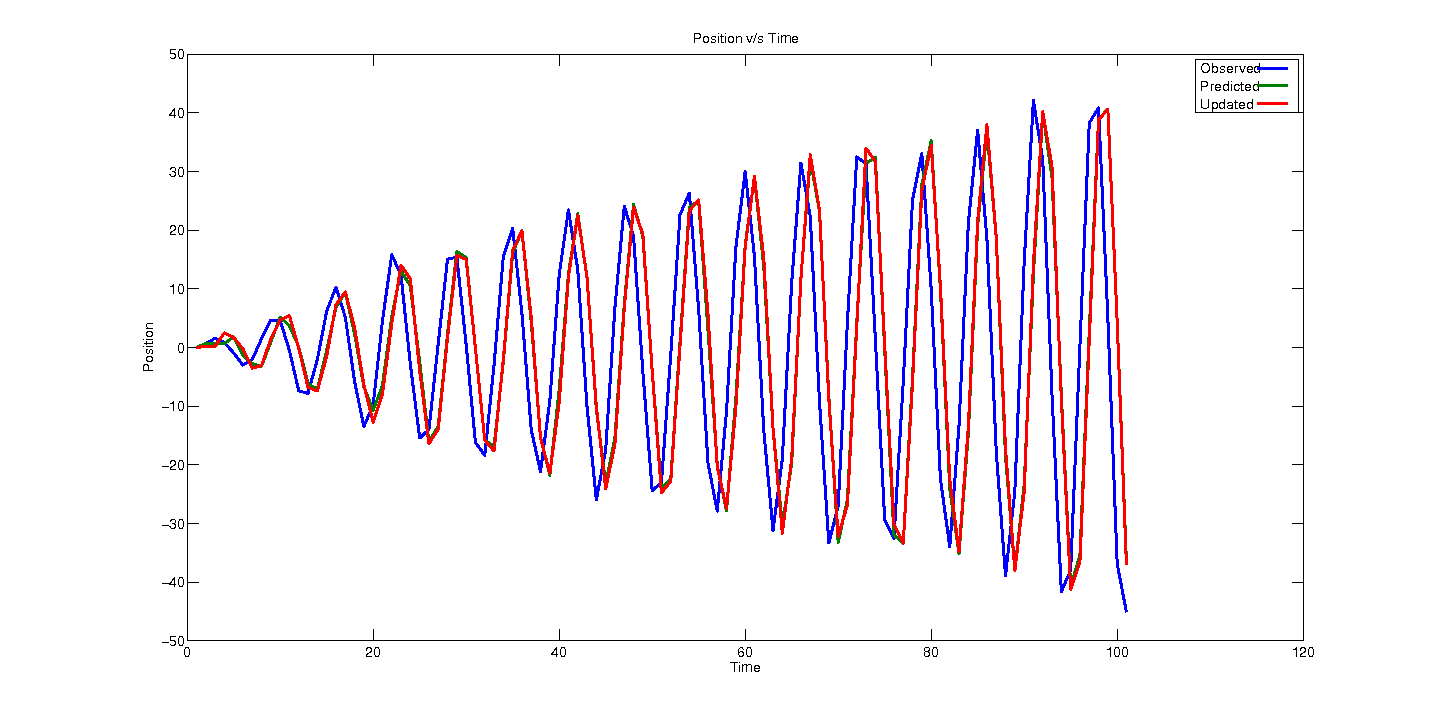
\includegraphics[width=\linewidth]{kalman-position-damping}
    \caption{Measured, predicted, filtered position with damping and resonance}
\end{figure}

\begin{figure}
    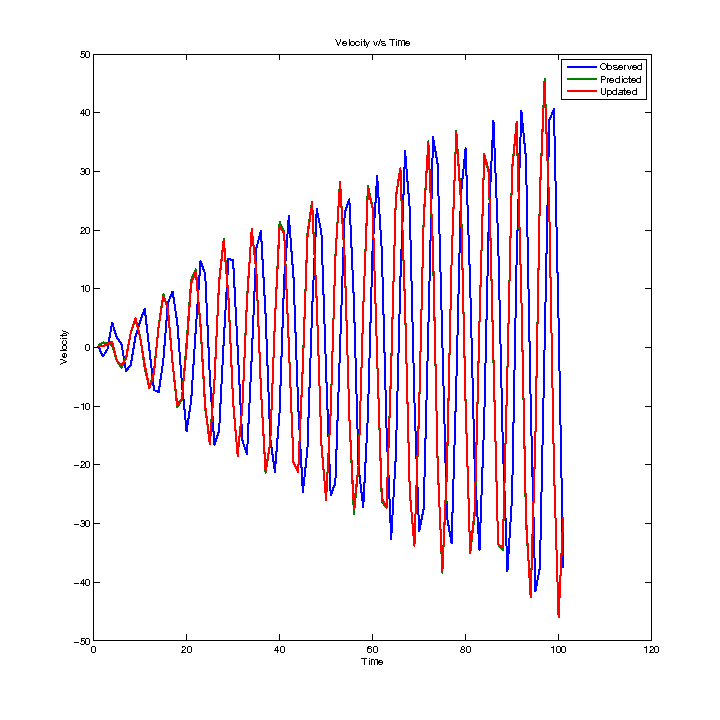
\includegraphics[width=\linewidth]{kalman-velocity-damping}
    \caption{Measured, predicted, filtered velocity with damping and resonance}
\end{figure}

\begin{figure}
    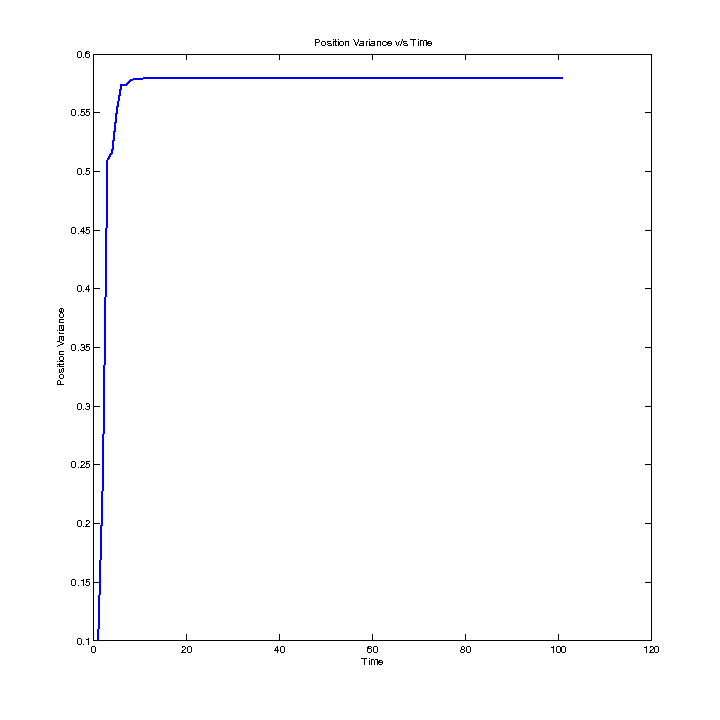
\includegraphics[width=\linewidth]{kalman-variance1-damping}
    \caption{Position variance with damping and resonance}
\end{figure}

\begin{figure}
    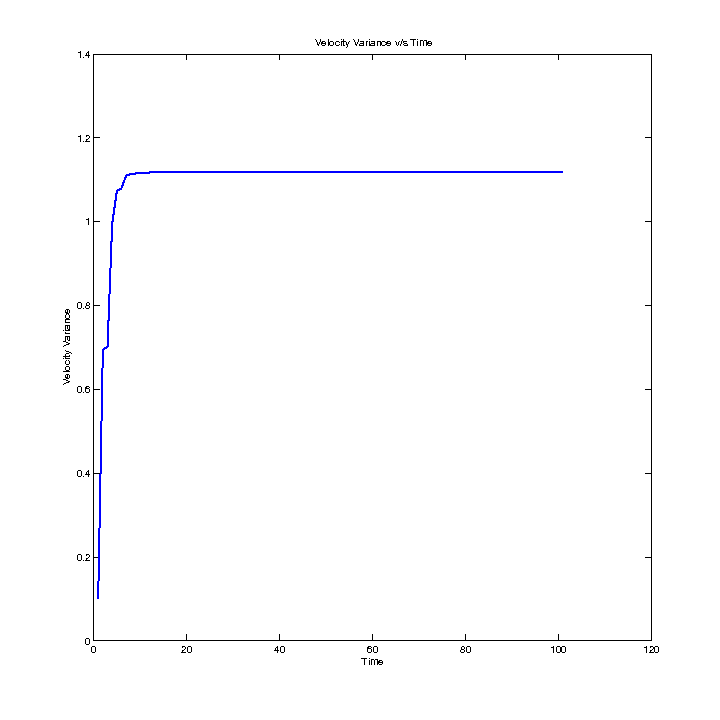
\includegraphics[width=\linewidth]{kalman-variance2-damping}
    \caption{Velocity variance with damping and resonance}
\end{figure}


For $m=100,c=1,k=1,b=1, Var(\omega)=0.1, Var(\epsilon)=0.1$


\begin{figure}
    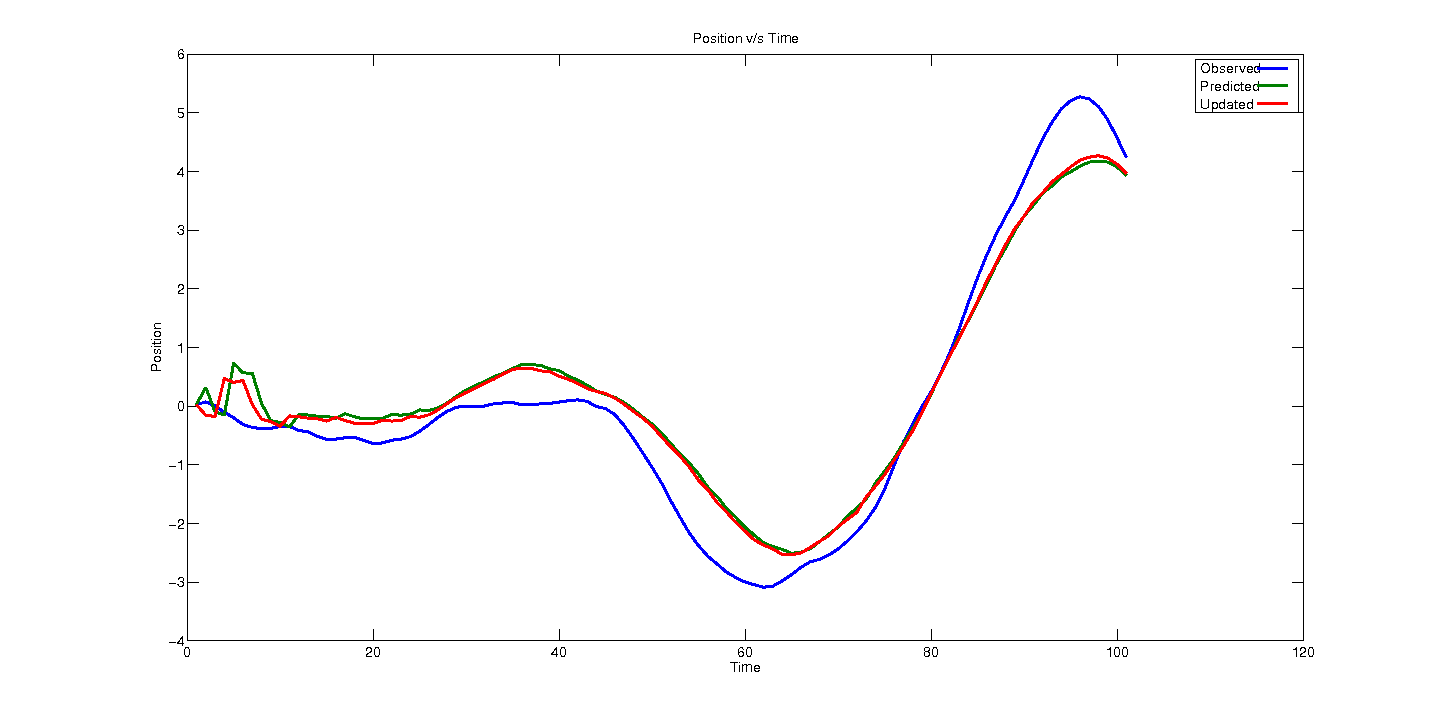
\includegraphics[width=\linewidth]{kalman-position-m100}
    \caption{Measured, predicted, filtered position with high mass}
\end{figure}

\begin{figure}
    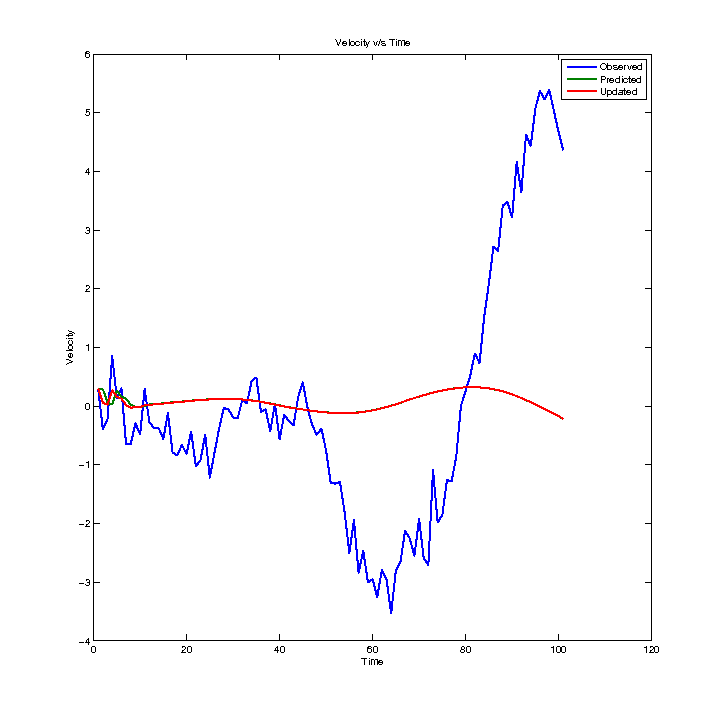
\includegraphics[width=\linewidth]{kalman-velocity-m100}
    \caption{Measured, predicted, filtered velocity with high mass}
\end{figure}

\begin{figure}
    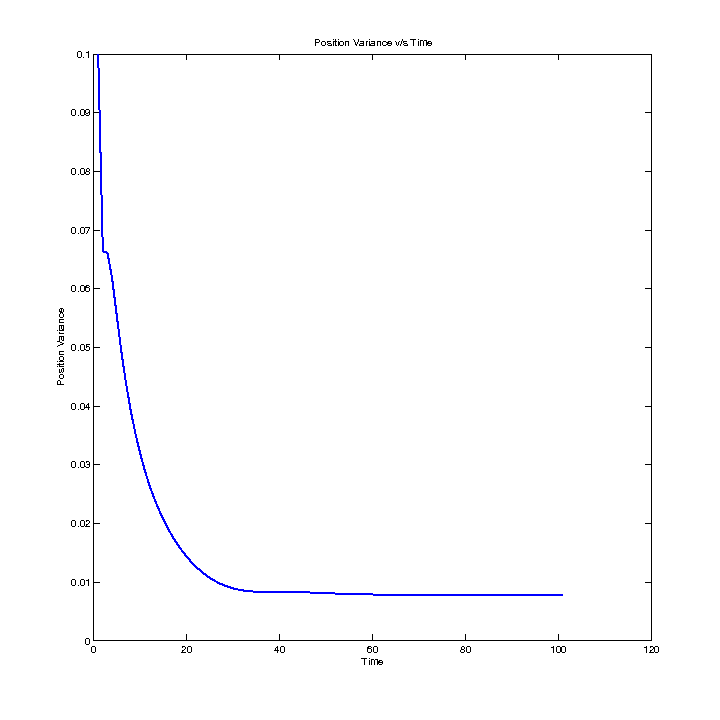
\includegraphics[width=\linewidth]{kalman-variance1-m100}
    \caption{Position variance with high mass}
\end{figure}

\begin{figure}
    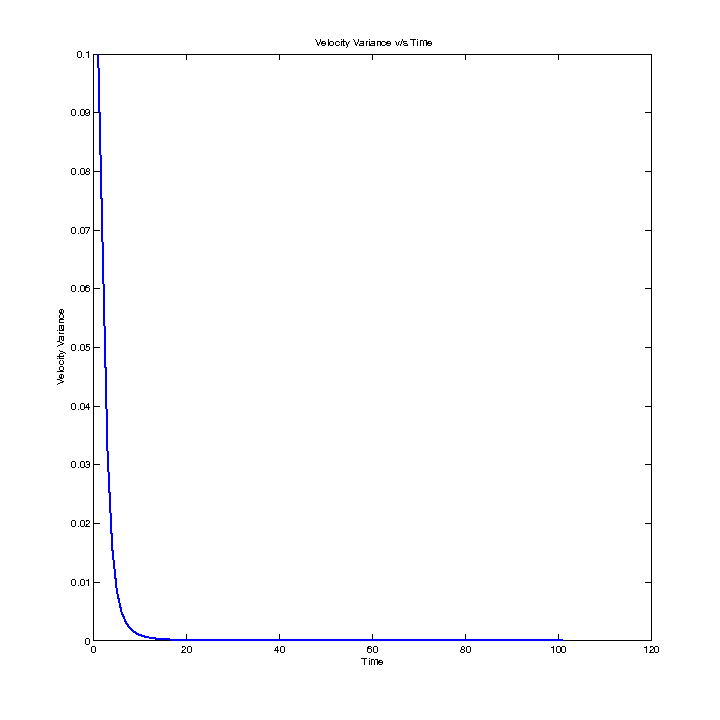
\includegraphics[width=\linewidth]{kalman-variance2-m100}
    \caption{Velocity variance with high mass}
\end{figure}


For $m=1,c=1,k=1,b=1, Var(\omega)=0.1, Var(\epsilon)=0.1$


\begin{figure}
    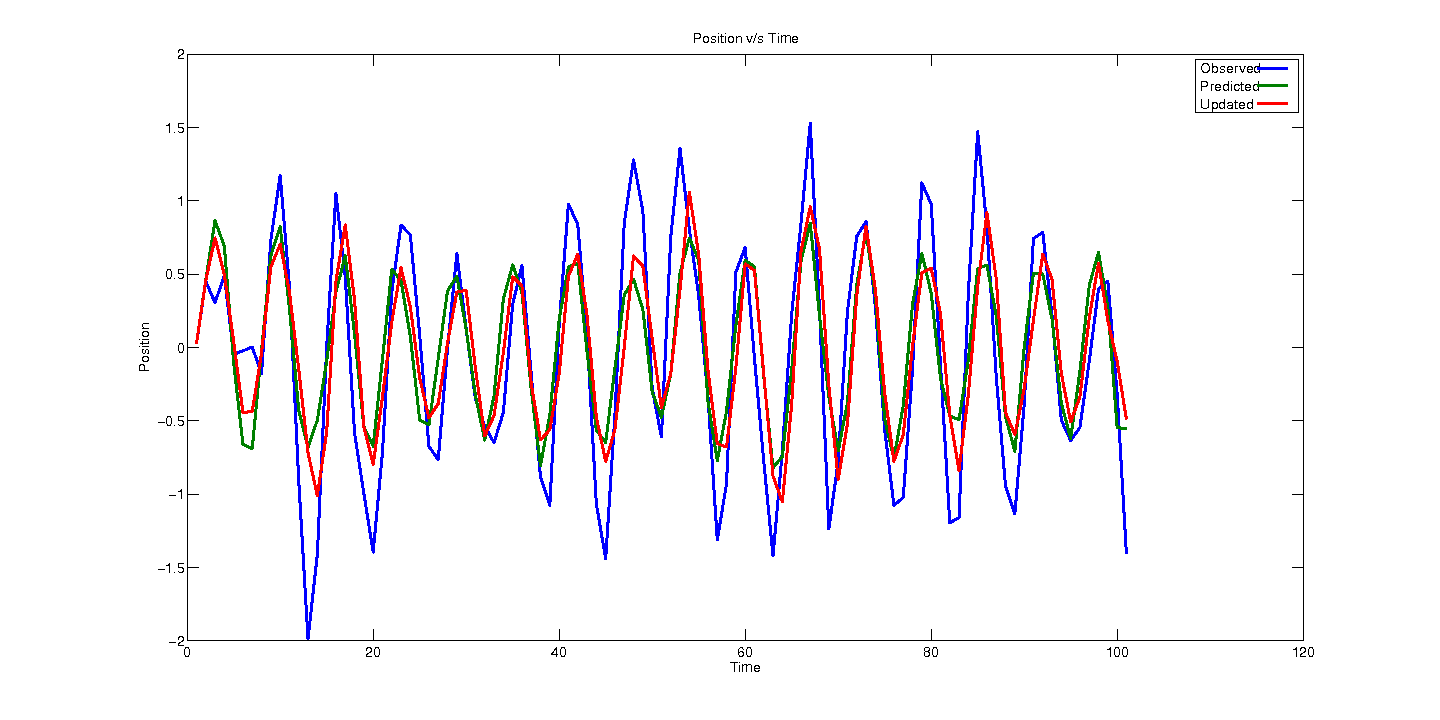
\includegraphics[width=\linewidth]{kalman-position-m1}
    \caption{Measured, predicted, filtered position with low mass}
\end{figure}

\begin{figure}
    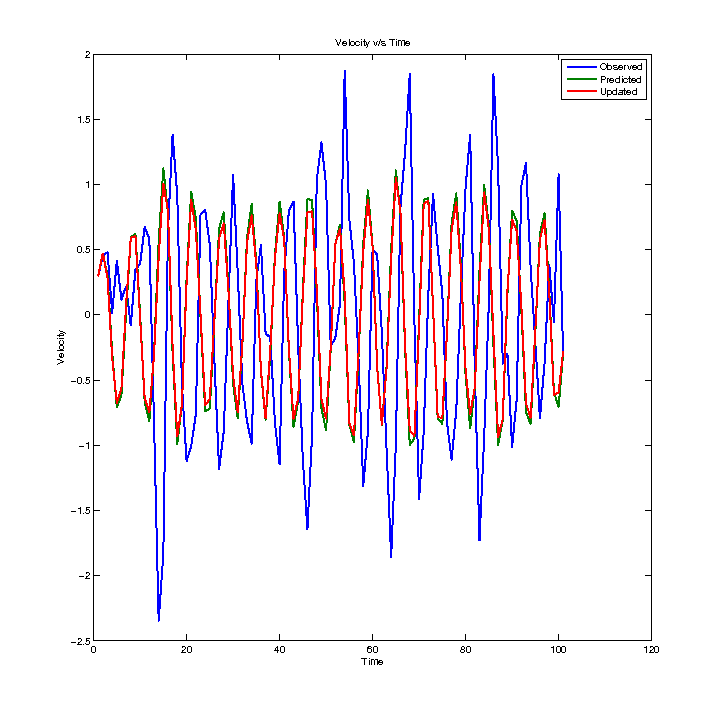
\includegraphics[width=\linewidth]{kalman-velocity-m1}
    \caption{Measured, predicted, filtered velocity with low mass}
\end{figure}

\begin{figure}
    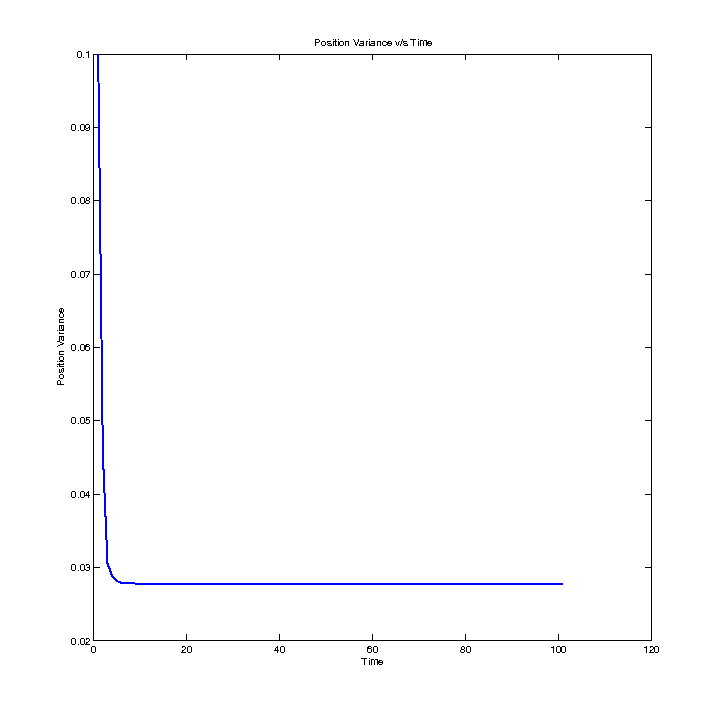
\includegraphics[width=\linewidth]{kalman-variance1-m1}
    \caption{Position variance with low mass}
\end{figure}

\begin{figure}
    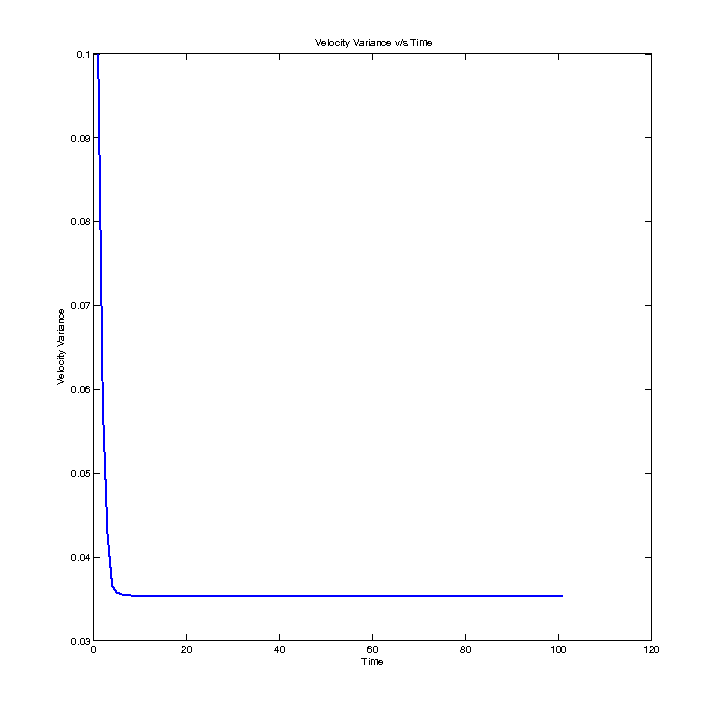
\includegraphics[width=\linewidth]{kalman-variance2-m1}
    \caption{Velocity variance with low mass}
\end{figure}


For $m=1,c=1,k=1,b=1, Var(\omega)=2, Var(\epsilon)=2$


\begin{figure}
    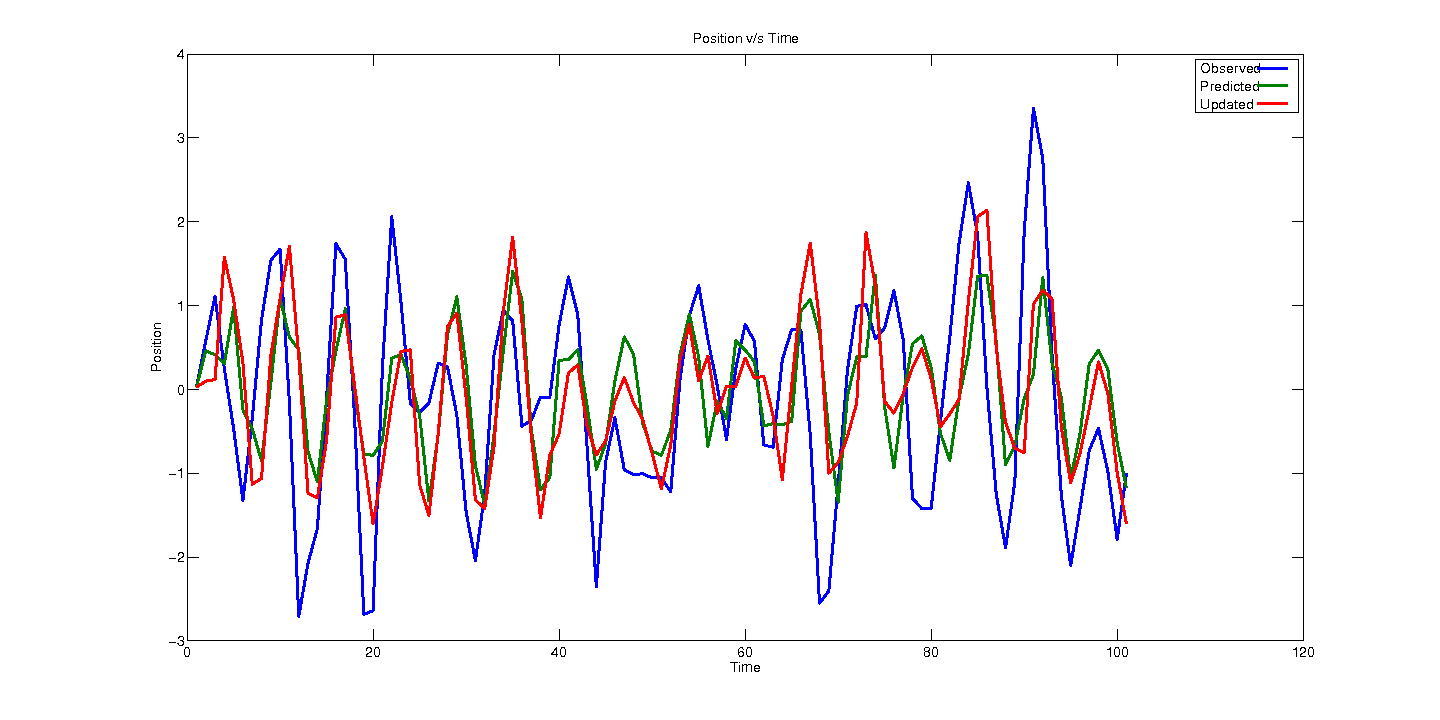
\includegraphics[width=\linewidth]{kalman-position-m1h}
    \caption{Measured, predicted, filtered position with low mass high variance}
\end{figure}

\begin{figure}
    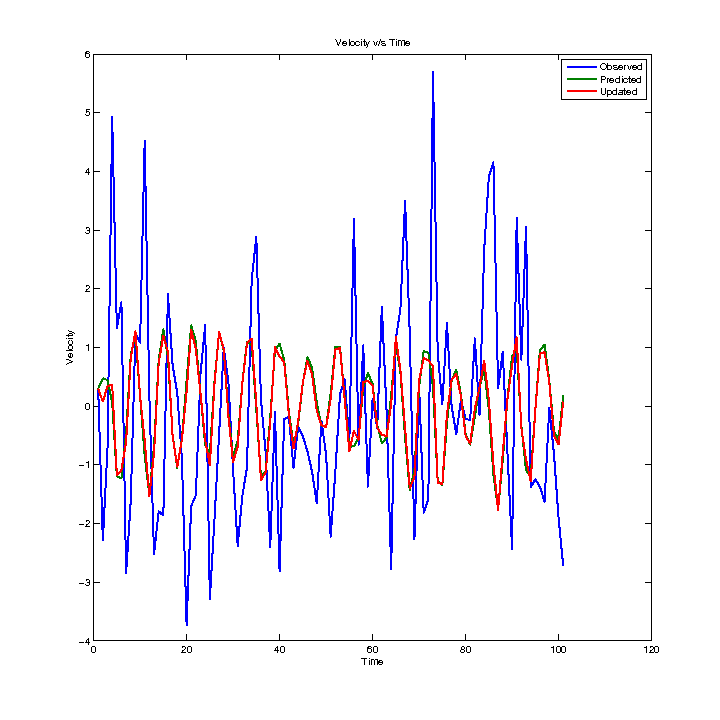
\includegraphics[width=\linewidth]{kalman-velocity-m1h}
    \caption{Measured, predicted, filtered velocity with low mass high variance}
\end{figure}

\begin{figure}
    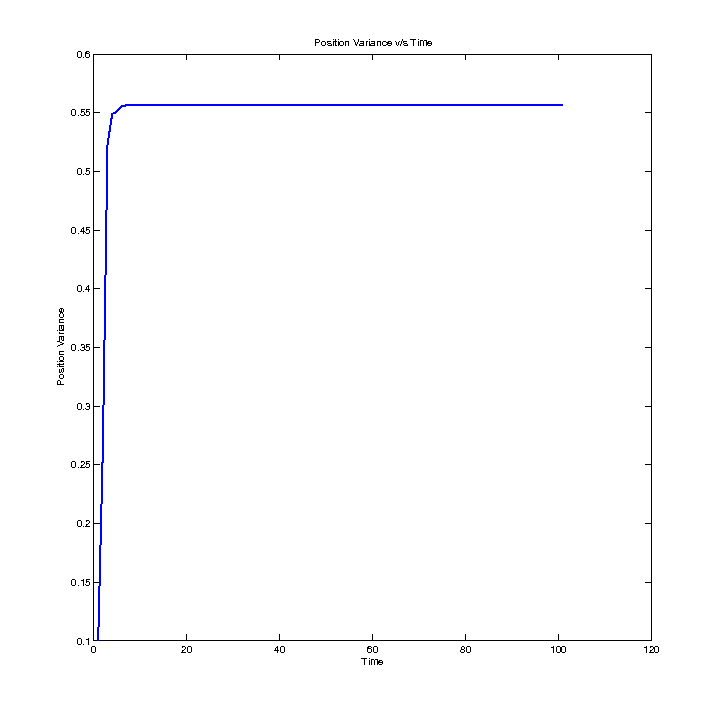
\includegraphics[width=\linewidth]{kalman-variance1-m1h}
    \caption{Position variance with low mass high variance}
\end{figure}

\begin{figure}
    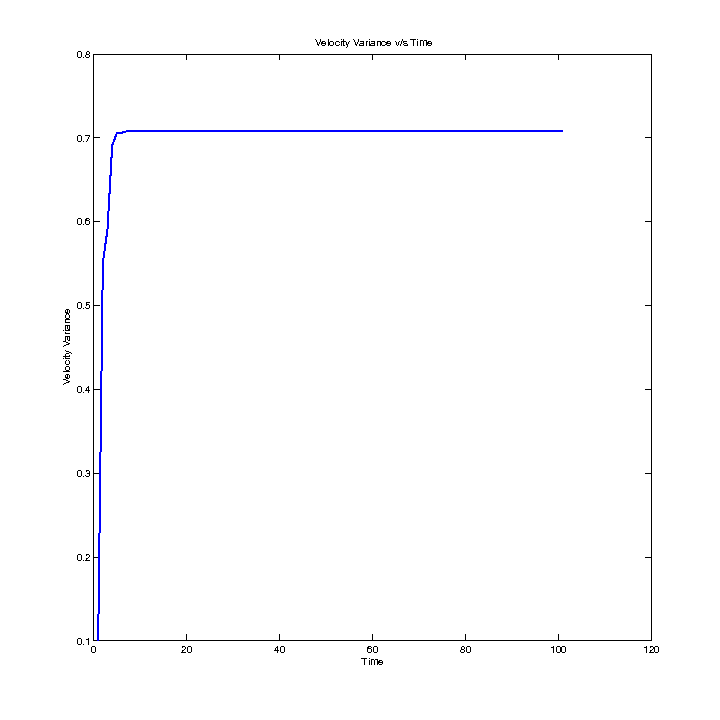
\includegraphics[width=\linewidth]{kalman-variance2-m1h}
    \caption{Velocity variance with low mass high variacne}
\end{figure}


\end{document}
